\documentclass[11pt,a4paper]{article}

% =============================================================================
% PREÁMBULO Y PAQUETES DE CONFIGURACIÓN
% =============================================================================
\usepackage[utf8]{inputenc}
\usepackage[spanish, es-tabla]{babel}
\usepackage{amsmath, amssymb, amsfonts}
\usepackage{geometry}
\geometry{top=2.5cm, bottom=2.5cm, left=2.5cm, right=2.5cm}

% Tipografía y estética profesional
\usepackage{lmodern}
\usepackage{microtype}
\usepackage{booktabs}
\usepackage{array}
\usepackage{graphicx}
\usepackage{xcolor}
\usepackage{enumitem}

% Figuras y listados de código
\usepackage{tikz}
\usetikzlibrary{patterns, arrows.meta}
\usepackage{listings}
\lstset{
    basicstyle=\ttfamily\footnotesize,
    keywordstyle=\color{blue!60!black}\bfseries,
    commentstyle=\color{gray}\itshape,
    stringstyle=\color{red!50!black},
    numbers=left, numberstyle=\tiny\color{gray}, numbersep=8pt,
    frame=single, rulecolor=\color{gray!60},
    breaklines=true, showstringspaces=false, tabsize=4,
    inputencoding=utf8, extendedchars=true,
    literate=
      {á}{{\'a}}1 {é}{{\'e}}1 {í}{{\'i}}1 {ó}{{\'o}}1 {ú}{{\'u}}1
      {Á}{{\'A}}1 {É}{{\'E}}1 {Í}{{\'I}}1 {Ó}{{\'O}}1 {Ú}{{\'U}}1
      {ñ}{{\~n}}1 {Ñ}{{\~N}}1 {ü}{{\"u}}1 {¿}{{?`}}1 {¡}{{!`}}1
      {ω}{{$\omega$}}1 {ρ}{{$\rho$}}1 {π}{{$\pi$}}1 {η}{{$\eta$}}1
      {γ}{{$\gamma$}}1 {φ}{{$\phi$}}1 {σ}{{$\sigma$}}1 {Λ}{{$\Lambda$}}1
      {Ω}{{$\Omega$}}1 {∫}{{$\int$}}1 {∇}{{$\nabla$}}1 {∂}{{$\partial$}}1
      {−}{{-}}1 {·}{{$\cdot$}}1 {²}{{$^2$}}1 {≥}{{$\geq$}}1 {≤}{{$\leq$}}1
      {→}{{$\rightarrow$}}1 {←}{{$\leftarrow$}}1 {Δ}{{$\Delta$}}1
      {═}{{=}}1 {─}{{-}}1 {μ}{{$\mu$}}1 {ε}{{$\epsilon$}}1,
}

% Cajas elegantes estilo apunte de clase (Estilo Dr. Rodolfo Venegas / UACh)
\usepackage[many]{tcolorbox}
\newtcolorbox{resumenbox}{
    colback=gray!6!white,
    colframe=gray!50!black,
    arc=2mm,
    boxrule=0.7pt,
    left=12pt, right=12pt, top=10pt, bottom=10pt,
    title=\textbf{\large Resumen Ejecutivo},
    coltitle=white
}

\newtcolorbox{infobox}[1]{
    colback=blue!4!white,
    colframe=blue!45!black,
    arc=1.5mm,
    boxrule=0.6pt,
    title=\textbf{#1},
    fonttitle=\bfseries\small
}

% Encabezados y pies de página
\usepackage{fancyhdr}
\pagestyle{fancy}
\fancyhf{}
\setlength{\headheight}{22pt}
\renewcommand{\headrulewidth}{0.5pt}
\renewcommand{\footrulewidth}{0.4pt}

\fancyhead[L]{\small\textbf{Materiales Acústicos} -- Memoria de Titulación}
\fancyhead[R]{\small UACh -- Valdivia, Chile}
\fancyfoot[L]{\small\textit{Álvaro Flores Varas -- FEniCSx, TMM \& ISO 10534-2}}
\fancyfoot[R]{\thepage}

% Formato equilibrado de títulos de sección
\usepackage{titlesec}
\titleformat{\section}{\large\bfseries\color{blue!40!black}}{\thesection.}{0.6em}{}[\titlerule]
\titleformat{\subsection}{\normalfont\bfseries\color{black!85}}{\thesubsection.}{0.5em}{}
\titleformat{\subsubsection}{\normalfont\bfseries\itshape\color{black!75}}{\thesubsubsection.}{0.5em}{}
\titlespacing*{\section}{0pt}{1.5em}{0.8em}
\titlespacing*{\subsection}{0pt}{1.2em}{0.5em}
\titlespacing*{\subsubsection}{0pt}{0.8em}{0.4em}

\usepackage{hyperref}
\hypersetup{
    colorlinks=true,
    linkcolor=blue!50!black,
    citecolor=blue!50!black,
    urlcolor=blue!50!black
}

% =============================================================================
% INICIO DEL DOCUMENTO
% =============================================================================
\begin{document}

% BLOQUE DE TÍTULO ACADÉMICO HARMÓNICO
\begin{center}
    {\Large \bfseries Caracterización de Parámetros Acústicos de Materiales Porosos} \\[0.4em]
    {\large \bfseries mediante FEniCSx, TMM y el Método de Dos Cavidades (ISO 10534-2)} \\[1.2em]
    
    \textbf{Autor:} Álvaro Flores Varas \\[0.5em]
    \small
    \textbf{Docentes Guías:} Ph.D. Uwe Mülich \quad $\cdot$ \quad Ph.D. Rodolfo Venegas \\[0.2em]
    \textbf{Docente Informante:} Ph.D. Daniel Sánchez \\[0.6em]
    
    \textit{Escuela de Ingeniería en Construcción -- Universidad Austral de Chile (UACh)} \\[0.2em]
    Valdivia, Chile \quad $\cdot$ \quad \today
\end{center}

\vspace{0.5em}

\begin{resumenbox}
Esta investigación presenta la caracterización acústica de materiales porosos absorbentes mediante un enfoque integrado en tres niveles: modelación analítica directa mediante el \textbf{Método de Matrices de Transferencia (TMM)}, simulación numérico-variacional por elementos finitos en \textbf{FEniCSx/DOLFINx} respetando la normativa \textbf{ISO 10534-2} (método de función de transferencia con dos micrófonos), y caracterización inversa mediante el \textbf{Método de Dos Cavidades (Utsuno et al., 1989)}. Asumiendo un esqueleto sólido rígido e inamovible, el medio heterogéneo se homogeneiza como un fluido equivalente dependiente de la frecuencia a partir de los 5 parámetros microestructurales del modelo de \textbf{Johnson-Champoux-Allard (JCA)}, garantizando la continuidad de fase en el número de onda $k_c(\omega)$.
\end{resumenbox}

\vspace{1em}

% =============================================================================
% SECCIÓN 1: MARCO TEÓRICO ANALÍTICO Y FÍSICA DEL FLUIDO EQUIVALENTE
% =============================================================================
\section{Marco Teórico Analítico}
\label{sec:marco}

\subsection{Fundamentos de la Propagación en Aire Libre}

En un fluido ideal no viscoso en reposo (aire libre), las pequeñas perturbaciones de presión $p$ y densidad $\rho$ cumplen un proceso de compresión adiabático e isentrópico. El módulo de compresibilidad volumétrico del aire $K_0$ representa la respuesta elástica o rigidez del fluido ante variaciones volumétricas:

\begin{equation}
K_0 = \rho_0 \left( \frac{\partial P}{\partial \rho} \right)_s = \gamma P_0
\end{equation}

donde $\rho_0$ es la densidad del aire en reposo, $P_0$ es la presión atmosférica y $\gamma = 1{,}4$ es el coeficiente de expansión adiabática. La celeridad del sonido $c_0$ y el número de onda $k_0$ se expresan como:

\begin{equation}
c_0 = \sqrt{\frac{K_0}{\rho_0}}, \qquad k_0^2 = \frac{\omega^2}{c_0^2} = \frac{\omega^2 \rho_0}{K_0}
\end{equation}

\subsection{Homogeneización y Concepto de Fluido Equivalente en Poros}

En un material poroso real, la geometría interna consiste en una red compleja de poros con paredes sólidas y rugosas. Al penetrar una onda sonora en el material:
\begin{enumerate}[label=\arabic*.]
    \item \textbf{Pérdidas Viscosas:} El aire roza contra las paredes sólidas de los poros, generando fricción viscosa en la capa límite.
    \item \textbf{Pérdidas Térmicas:} Las paredes sólidas actúan como un disipador térmico debido al estrecho diámetro de las cavidades. El calor generado por la compresión del aire se transfiere a la matriz sólida, rompiendo la condición adiabática pura y produciendo un comportamiento politrópico o isotérmico a bajas frecuencias.
\end{enumerate}

Bajo la hipótesis de \textbf{marco o esqueleto rígido} (donde la matriz sólida no vibra ni se acopla elásticamente con la onda), la teoría de homogeneización permite preservar la estructura funcional de la ecuación de Helmholtz, reemplazando $K_0$ y $\rho_0$ por \textbf{propiedades efectivas complejas dependientes de la frecuencia angular} $\omega$:

\begin{equation}
c_{eq}(\omega) = \sqrt{\frac{K_{eq}(\omega)}{\rho_{eq}(\omega)}}, \qquad k_c(\omega) = \omega \sqrt{\frac{\rho_{eq}(\omega)}{K_{eq}(\omega)}}, \qquad Z_c(\omega) = \sqrt{\rho_{eq}(\omega) \cdot K_{eq}(\omega)}
\end{equation}

\subsection{El Modelo de Johnson-Champoux-Allard (JCA)}

El modelo semi-fenomenológico JCA parametriza $\rho_{eq}(\omega)$ y $K_{eq}(\omega)$ mediante 5 propiedades físicas no acústicas e independientes de la frecuencia:

\subsubsection{Física de la Densidad Dinámica $\rho_{eq}(\omega)$ (Johnson et al., 1987)}
Johnson analizó la transición entre dos regímenes visco-inerciales:
\begin{itemize}
    \item \textbf{Bajas Frecuencias ($\omega \to 0$):} La capa límite viscosa ocupa todo el poro. El fluido se mueve pegado a las paredes y la \textbf{resistividad al flujo estático ($\sigma$)} domina por completo.
    \item \textbf{Altas Frecuencias ($\omega \to \infty$):} La capa límite viscosa se reduce. El fluido en el centro del poro se mueve por inercia. La \textbf{tortuosidad ($\alpha_\infty$)} incrementa la inercia efectiva al alargar la trayectoria de las líneas de corriente, mientras que la \textbf{longitud característica viscosa ($\Lambda_v$)} pondera el tamaño de los poros donde ocurre el rozamiento.
\end{itemize}

\begin{infobox}{Densidad Dinámica Equivalente $\rho_{eq}(\omega)$}
\begin{equation}
\rho_{eq}(\omega) = \frac{\rho_0 \alpha_\infty}{\phi} \left[ 1 - j \frac{\sigma \phi}{\omega \rho_0 \alpha_\infty} \sqrt{1 + j \frac{4 \alpha_\infty^2 \eta \rho_0 \omega}{\sigma^2 \phi^2 \Lambda_v^2}} \right]
\end{equation}
\end{infobox}

\subsubsection{Física del Módulo de Compresibilidad $K_{eq}(\omega)$ (Champoux \& Allard, 1991)}
Champoux y Allard introdujeron la \textbf{longitud característica térmica ($\Lambda_t$)} para describir los intercambios de calor:
\begin{itemize}
    \item \textbf{Bajas Frecuencias:} Existe tiempo suficiente para el intercambio térmico entre aire y sólido (proceso isotérmico, $K \to P_0/\phi$).
    \item \textbf{Altas Frecuencias:} El ciclo es demasiado rápido para permitir la transferencia de calor (proceso adiabático, $K \to \gamma P_0/\phi$).
\end{itemize}

\begin{infobox}{Módulo de Compresibilidad Dinámico $K_{eq}(\omega)$}
\begin{equation}
K_{eq}(\omega) = \frac{\gamma P_0 / \phi}{\gamma - (\gamma - 1) \left[ 1 - j \frac{8 \eta}{\omega \rho_0 \operatorname{Pr} \Lambda_t^2} \sqrt{1 + j \frac{\omega \rho_0 \operatorname{Pr} \Lambda_t^2}{16 \eta}} \right]^{-1}}
\end{equation}
\end{infobox}

% =============================================================================
% SECCIÓN 2: MÉTODO DE MATRICES DE TRANSFERENCIA (TMM)
% =============================================================================
\section{Método de Matrices de Transferencia (TMM)}

El Método de Matrices de Transferencia (\textit{Transfer Matrix Method}, TMM) relaciona las variables de estado acústico (presión $p$ y velocidad de partícula $v$) entre la entrada ($x=0$) y la salida ($x=L$) de una capa homogénea.

\subsection{Deducción Unidimensional a partir de la Ecuación de Euler}

Asumiendo una dependencia temporal armónica $e^{+j\omega t}$, las perturbaciones de presión $p(x,t)$ y velocidad $v(x,t)$ se expresan como:
\begin{equation}
p(x,t) = p(x) e^{j\omega t}, \qquad v(x,t) = v(x) e^{j\omega t}
\end{equation}

La solución general espacial de la presión $p(x)$ es:
\begin{equation}
p(x) = A e^{-j k x} + B e^{+j k x}
\label{eq:presion_solucion}
\end{equation}

La conservación del momento lineal 1D (Ecuación de Euler sin fuerzas de cuerpo) establece:
\begin{equation}
\rho_0 \frac{\partial v(x,t)}{\partial t} = -\frac{\partial p(x,t)}{\partial x} \implies j \omega \rho_0 v(x) = -\frac{d p(x)}{d x}
\end{equation}

Derivando la Ecuación~(\ref{eq:presion_solucion}) respecto a $x$ y sustituyendo:
\begin{equation}
j \omega \rho_0 v(x) = j k \left( A e^{-j k x} - B e^{+j k x} \right) \implies v(x) = \frac{k}{\omega \rho_0} \left( A e^{-j k x} - B e^{+j k x} \right)
\end{equation}

Puesto que $Z_c = \rho_0 c = \frac{\omega \rho_0}{k}$, se concluye que $\frac{1}{Z_c} = \frac{k}{\omega \rho_0}$, dando lugar a:
\begin{equation}
v(x) = \frac{1}{Z_c} \left( A e^{-j k x} - B e^{+j k x} \right)
\label{eq:velocidad_solucion}
\end{equation}

\subsection{Construcción de la Matriz de Transferencia TMM}

Evaluando las Ecuaciones~(\ref{eq:presion_solucion}) y (\ref{eq:velocidad_solucion}) en $x=0$ y $x=L$, y despejando las amplitudes $A$ y $B$ en función de la salida $[p(L), v(L)]^T$:
\begin{equation}
A = \frac{1}{2} \left[ p(L) + Z_c v(L) \right] e^{+j k L}, \qquad B = \frac{1}{2} \left[ p(L) - Z_c v(L) \right] e^{-j k L}
\end{equation}

Sustituyendo en $p(0) = A + B$ y $v(0) = \frac{1}{Z_c}(A - B)$, y aplicando las identidades de Euler ($\cos\theta = \frac{e^{j\theta} + e^{-j\theta}}{2}$, $j\sin\theta = \frac{e^{j\theta} - e^{-j\theta}}{2}$):

\begin{infobox}{Matriz de Transferencia de Capa Homogénea}
\begin{equation}
\begin{bmatrix} p(0) \\ v(0) \end{bmatrix} = \mathbf{T} \begin{bmatrix} p(L) \\ v(L) \end{bmatrix} = \begin{bmatrix} \cos(k L) & j Z_c \sin(k L) \\ \frac{j}{Z_c} \sin(k L) & \cos(k L) \end{bmatrix} \begin{bmatrix} p(L) \\ v(L) \end{bmatrix}
\end{equation}
\end{infobox}

\subsection{Relación entre Impedancia de Superficie $Z_s$, Coeficiente de Reflexión $R$ y Absorción $\alpha$}

En $x = 0$, expresando las variables en función de las presiones incidentes $P_{in}$ y reflejadas $P_{out}$:
\begin{equation}
p(0) = P_{in} + P_{out}, \qquad v(0) = \frac{1}{Z_0} (P_{in} - P_{out})
\end{equation}

La impedancia de superficie $Z_s$ en $x=0$ resulta:
\begin{equation}
Z_s = \frac{p(0)}{v(0)} = Z_0 \left( \frac{P_{in} + P_{out}}{P_{in} - P_{out}} \right) = Z_0 \left( \frac{1 + R}{1 - R} \right)
\end{equation}

Despejando analíticamente el coeficiente de reflexión complejo $R = P_{out} / P_{in}$:
\begin{equation}
Z_s (1 - R) = Z_0 (1 + R) \implies R = \frac{Z_s - Z_0}{Z_s + Z_0} = \frac{T_{11} - Z_0 T_{21}}{T_{11} + Z_0 T_{21}}
\end{equation}

El coeficiente de absorción sonora $\alpha(\omega)$ en incidencia normal se define como:
\begin{equation}
\alpha(\omega) = 1 - |R(\omega)|^2 \qquad (0 \le \alpha \le 1)
\end{equation}

\subsection{Modelación del Sistema Bicapa y Continuidad Monocapa Trasera}

Para un sistema constituido por la muestra porosa de espesor $d$ ($\mathbf{T}_p$) y la cavidad de aire de espesor $L$ ($\mathbf{T}_a$):
\begin{equation}
\mathbf{T}^{tot} = \mathbf{T}_p(d) \cdot \mathbf{T}_a(L) \implies Z_s^{tot} = \frac{T_{11}^{tot}}{T_{21}^{tot}}
\end{equation}

En la interfaz $x = d$, la continuidad de presión y velocidad impone que la impedancia tras el poroso depende únicamente de la columna de aire:
\begin{equation}
Z(d) = Z_{aire}(L) = -j Z_0 \cot(k_0 L)
\end{equation}

% =============================================================================
% SECCIÓN 3: ALGORITMO INVERSO DE DOS CAVIDADES E INVERSIÓN CONTINUA DE FASE
% =============================================================================
\section{Algoritmo Inverso de Caracterización y Desenvolvimiento de Fase para $k_c$}
\label{sec:utsuno}

Al combinar dos ensayos independientes variando las cavidades traseras a $L_1$ y $L_2$, se conocen las impedancias monocapa $Z_1 = -j Z_0 \cot(k_0 L_1)$ y $Z_2 = -j Z_0 \cot(k_0 L_2)$, obteniendo las impedancias frontales $Z_{s1}$ y $Z_{s2}$.

\subsection{Impedancia Característica Reconstruida $Z_c(\omega)$}

\begin{infobox}{Impedancia Característica $Z_c(\omega)$ (Utsuno et al., 1989)}
\begin{equation}
Z_c(\omega) = \pm \sqrt{\frac{Z_{s1} Z_{s2} (Z_1 - Z_2) - Z_1 Z_2 (Z_{s1} - Z_{s2})}{(Z_1 - Z_2) - (Z_{s1} - Z_{s2})}}
\end{equation}
Se selecciona el signo positivo $(+)$ tal que $\operatorname{Re}(Z_c) > 0$ por la condición de pasividad.
\end{infobox}

\subsection{Número de Onda Complejo $k_c(\omega)$ y Desenvolvimiento Continuo de Fase}

A partir de la transformación de impedancias, se define el argumento complejo $\mathcal{X}(\omega)$:
\begin{equation}
\mathcal{X}(\omega) = \left( \frac{Z_{s1} + Z_c}{Z_{s1} - Z_c} \right) \left( \frac{Z_1 - Z_c}{Z_1 + Z_c} \right)
\end{equation}

El número de onda complejo se obtiene despejando la exponencial $e^{2 j k_c d} = \mathcal{X}(\omega)$ mediante el logaritmo natural complejo:
\begin{equation}
k_c(\omega) = \frac{1}{2 j d} \operatorname{Ln}\left( \mathcal{X}(\omega) \right) = \frac{1}{2 j d} \left( \ln |\mathcal{X}(\omega)| + j \arg(\mathcal{X}(\omega)) \right)
\end{equation}

\subsubsection{Garantía de Continuidad Suave mediante Unwrap}
Numéricamente, la función de argumento principal está acotada en el intervalo discontinuo $\arg(\mathcal{X}) \in [-\pi, \pi]$. Al barrer el rango de frecuencias $f$, cada vez que la fase cruza la frontera del plano complejo se genera un salto artificial discontinuo de $\pm 2\pi$.

Para garantizar la \textbf{continuidad suave y físicamente consistente} de las curvas de $\operatorname{Re}(k_c)$ e $\operatorname{Im}(k_c)$, se aplica el operador de desenvolvimiento continuo de fase (\textit{unwrap}):

\begin{infobox}{Número de Onda Complejo Continuo $k_c(\omega)$}
\begin{equation}
k_c(\omega) = \frac{1}{2 j d} \left( \ln |\mathcal{X}(\omega)| + j \cdot \operatorname{unwrap}\left( \arg(\mathcal{X}(\omega)) \right) \right)
\end{equation}
\end{infobox}

El procedimiento corregido de fase asegura que $\operatorname{Re}(k_c) > 0$ (propagación de fase hacia adelante) e $\operatorname{Im}(k_c) < 0$ (atenuación espacial por pérdidas visco-térmicas bajo la convención $e^{+j\omega t}$).

% =============================================================================
% SECCIÓN 4: FORMULACIÓN NUMÉRICA MEDIANTE EL MÉTODO DE ELEMENTOS FINITOS
% =============================================================================
\section{Formulación Numérica mediante el Método de Elementos Finitos (FEniCSx)}
\label{sec:fem}

La contraparte numérica de la caracterización consiste en simular el ensayo completo en el tubo de impedancia: se resuelve la ecuación de onda en el dominio de la frecuencia, se registra la presión en las posiciones de los dos micrófonos y se procesan estas señales como en un ensayo real según ISO 10534-2. De este modo, la reconstrucción de $Z_c$ y $k_c$ se realiza con exactamente el mismo algoritmo inverso de la Sección~\ref{sec:utsuno}, y la comparación con la vía analítica evalúa únicamente la formulación numérica.

\subsection{Configuración del ensayo y sistema de coordenadas}

El ensayo se idealiza como propagación de ondas planas en un tubo rígido de sección constante. El eje $x$ tiene su origen en la \textbf{cara frontal de la muestra} y crece hacia la cavidad (Figura~\ref{fig:esquema}). Las distancias de los micrófonos se miden hacia el lado de la fuente, por lo que sus posiciones son $x=-x_1$ (micrófono $M_1$) y $x=-x_2$ (micrófono $M_2$), con $x_1>x_2$ y separación $s=x_1-x_2$. A continuación se ubican la muestra porosa de espesor $d$ (con $0<x<d$) y la cavidad de aire de longitud $L$ (con $d<x<d+L$), cerrada por una pared rígida. Como el método de dos cavidades requiere dos ensayos, el problema se resuelve dos veces: con $L=L_1$ y con $L=L_2$.

\begin{figure}[ht]
\centering
\begin{tikzpicture}[>=Stealth, font=\small]
  % Regiones
  \fill[blue!6]   (0,0)   rectangle (4.2,1.3);
  \fill[orange!30](4.2,0) rectangle (5.9,1.3);
  \fill[blue!6]   (5.9,0) rectangle (8.0,1.3);
  \draw[thick] (0,0) rectangle (8.0,1.3);
  \draw[thick] (4.2,0) -- (4.2,1.3);
  \draw[thick] (5.9,0) -- (5.9,1.3);
  % Pared rígida
  \fill[pattern=north east lines] (8.0,0) rectangle (8.25,1.3);
  \draw[thick] (8.0,0) -- (8.0,1.3);
  % Textos de región
  \node at (3.05,0.5) {Aire (tubo)};
  \node at (5.05,0.65) {\shortstack{Poroso\\(JCA)}};
  \node at (6.95,0.65) {Cavidad $L$};
  % Onda incidente y reflejada
  \draw[->, very thick, red!70!black]  (0.15,0.95) -- (0.85,0.95) node[right] {$P_{in}$};
  \draw[<-, very thick, blue!70!black] (0.15,0.35) -- (0.85,0.35) node[right] {$P_{out}$};
  % Micrófonos
  \foreach \xm/\nm in {1.9/M_1, 2.9/M_2}{
    \fill (\xm,1.3) circle (2pt);
    \draw (\xm,1.3) -- (\xm,1.65);
    \node[left] at (\xm,1.5) {$\nm$};
  }
  % Cotas
  \draw[<->] (0,-0.45) -- (4.2,-0.45) node[midway, fill=white, inner sep=1pt] {$L_t$};
  \draw[<->] (4.2,-0.45) -- (5.9,-0.45) node[midway, fill=white, inner sep=1pt] {$d$};
  \draw[<->] (5.9,-0.45) -- (8.0,-0.45) node[midway, fill=white, inner sep=1pt] {$L$};
  \draw[<->] (2.9,2.05) -- (4.2,2.05) node[midway, fill=white, inner sep=1pt] {$x_2$};
  \draw[<->] (1.9,2.5)  -- (4.2,2.5)  node[midway, fill=white, inner sep=1pt] {$x_1$};
  \draw[dotted] (1.9,1.65) -- (1.9,2.5);
  \draw[dotted] (2.9,1.65) -- (2.9,2.05);
  \draw[dotted] (4.2,1.3)  -- (4.2,2.5);
  % Ejes
  \draw[dashed] (4.2,-0.75) -- (4.2,-0.5);
  \node[below] at (4.2,-0.75) {$x=0$};
  \node[below] at (5.9,-0.75) {$x=d$};
  \node[below] at (8.0,-0.75) {$x=d+L$};
  \node[below] at (0,-0.75) {$x=-L_t$};
  \draw[->] (8.4,-0.45) -- (9.1,-0.45) node[right] {$x$};
\end{tikzpicture}
\caption{Esquema del ensayo simulado (no está a escala). El origen $x=0$ coincide con la cara frontal de la muestra y los micrófonos se ubican en $x=-x_1$ y $x=-x_2$.}
\label{fig:esquema}
\end{figure}

Las propiedades del fluido equivalente son constantes por tramos, con $K_0=\rho_0 c_0^2$:
\begin{equation}
\bigl(\rho(x),\,K(x)\bigr)=
\begin{cases}
\bigl(\rho_0,\;K_0\bigr), & -L_t<x<0 \quad \text{(aire del tubo)},\\[2pt]
\bigl(\rho_{eq}(\omega),\;K_{eq}(\omega)\bigr), & 0<x<d \quad \text{(muestra porosa)},\\[2pt]
\bigl(\rho_0,\;K_0\bigr), & d<x<d+L \quad \text{(cavidad de aire)}.
\end{cases}
\end{equation}
donde $\rho_{eq}(\omega)$ y $K_{eq}(\omega)$ son las ecuaciones del modelo JCA de la Sección~\ref{sec:marco}, alimentadas por los cinco parámetros no acústicos $(\phi,\sigma,\alpha_\infty,\Lambda_v,\Lambda_t)$. Esto garantiza que la vía analítica (TMM) y la numérica (FEM) parten exactamente del mismo material.

\subsection{Ecuaciones gobernantes y ecuación de Helmholtz}

Se parte de las ecuaciones linealizadas de la acústica para un fluido ideal (sin viscosidad ni conducción de calor, perturbaciones pequeñas y compresión adiabática, $p=c_0^2\rho'$). La compresibilidad del medio queda contenida en la ecuación de continuidad, y la inercia en la de Euler:
\begin{align}
\frac{1}{c_0^2}\frac{\partial p}{\partial t} + \rho_0\,\nabla\!\cdot\mathbf{v} &= 0, \label{eq:continuidad}\\
\rho_0\,\frac{\partial \mathbf{v}}{\partial t} &= -\nabla p. \label{eq:euler}
\end{align}
Con dependencia temporal armónica $p(\mathbf{x},t)=p(\mathbf{x})e^{j\omega t}$ y $\mathbf{v}(\mathbf{x},t)=\mathbf{v}(\mathbf{x})e^{j\omega t}$, donde $\mathbf{x}$ es el vector posición, se cumple $\partial p/\partial t = j\omega\,p\,e^{j\omega t}$, $\partial\mathbf{v}/\partial t=j\omega\,\mathbf{v}\,e^{j\omega t}$ y $\nabla p(\mathbf{x},t)=\nabla p(\mathbf{x})\,e^{j\omega t}$. Eliminando el factor $e^{j\omega t}$:
\begin{equation}
\frac{j\omega}{c_0^2}\,p + \rho_0\nabla\!\cdot\mathbf{v}=0, \qquad j\omega\rho_0\,\mathbf{v}=-\nabla p \;\;\Longrightarrow\;\; \mathbf{v}=-\frac{1}{j\omega\rho_0}\nabla p .
\end{equation}
Sustituyendo $\mathbf{v}$ en la continuidad se obtiene:
\begin{equation}
\frac{j\omega}{c_0^2}\,p-\frac{1}{j\omega}\nabla^2 p=0
\;\Longrightarrow\;
\nabla^2 p + k_0^2\,p=0
\;\Longrightarrow\;
\nabla\!\cdot\!\left(\frac{1}{\rho_0}\nabla p\right)+\frac{\omega^2}{K_0}\,p=0,
\end{equation}
donde se usó $k_0^2/\rho_0=\omega^2/(\rho_0c_0^2)=\omega^2/K_0$. La última forma es la adecuada para medios heterogéneos, pues permite que $\rho$ y $K$ varíen en el espacio. Bajo el concepto de fluido equivalente se reemplazan $\rho_0\to\rho_{eq}(\omega)$ y $K_0\to K_{eq}(\omega)$ en la muestra porosa:
\begin{infobox}{Forma fuerte: Helmholtz para el fluido equivalente}
\begin{equation}
\nabla\!\cdot\!\left(\frac{1}{\rho(\mathbf{x})}\,\nabla p\right)+\frac{\omega^2}{K(\mathbf{x})}\,p=0 \qquad \text{en } \Omega .
\label{eq:fuerte}
\end{equation}
\end{infobox}

\subsection{Forma débil}

Se multiplica la Ecuación~(\ref{eq:fuerte}) por una función de test $q$ y se integra sobre el dominio $\Omega$:
\begin{equation}
\int_\Omega \nabla\!\cdot\!\left(\frac{1}{\rho}\nabla p\right) q \, d\Omega + \int_\Omega \frac{\omega^2}{K}\,p\,q \, d\Omega = 0 .
\end{equation}
Definiendo $\mathbf{Q}=\frac{1}{\rho}\nabla p$, se usa la identidad $\nabla\!\cdot(\mathbf{Q}q)=(\nabla\!\cdot\mathbf{Q})\,q+\mathbf{Q}\cdot\nabla q$, es decir, $(\nabla\!\cdot\mathbf{Q})\,q=\nabla\!\cdot(\mathbf{Q}q)-\mathbf{Q}\cdot\nabla q$. Aplicando el teorema de la divergencia (Gauss), $\int_\Omega \nabla\!\cdot(\mathbf{Q}q)\,d\Omega=\oint_{\partial\Omega}(\mathbf{Q}\cdot\mathbf{n})\,q\,ds$, resulta:
\begin{equation}
-\int_\Omega \frac{1}{\rho}\,\nabla p\cdot\nabla q\,d\Omega
+\int_\Omega \frac{\omega^2}{K}\,p\,q\,d\Omega
+\oint_{\partial\Omega}\frac{1}{\rho}\,\frac{\partial p}{\partial n}\,q\,ds = 0 ,
\label{eq:debil_general}
\end{equation}
con $\partial p/\partial n=\nabla p\cdot\mathbf{n}$ y $\mathbf{n}$ la normal exterior unitaria. Los efectos de las fronteras entran únicamente a través del último término, que se evalúa con las condiciones de contorno del problema.

\subsection{Condiciones de contorno}

\subsubsection{Extremo izquierdo: radiación con fuente (Sommerfeld no homogénea)}

En el extremo izquierdo del tubo la presión es la suma de la onda incidente $P_{in}$ (amplitud conocida, impuesta por la fuente) y de la onda reflejada $P_{out}$ (desconocida, pues depende de la absorción de la muestra): $p=P_{in}+P_{out}$. Como la presión solo varía en $x$, $\nabla p=(\partial p/\partial x,0,0)$, y con $p(x)=Ae^{-jk_0x}+Be^{+jk_0x}$ se tiene $\partial p/\partial x=-jk_0P_{in}+jk_0P_{out}$. La normal exterior en el extremo izquierdo es $\mathbf{n}=(-1,0,0)$, por lo que
\begin{equation}
\frac{\partial p}{\partial n}=-\frac{\partial p}{\partial x}=jk_0P_{in}-jk_0P_{out}.
\end{equation}
FEniCSx no conoce $P_{out}$, pero esta se elimina con $P_{out}=p-P_{in}$:
\begin{equation}
\frac{\partial p}{\partial n}=jk_0P_{in}-jk_0\,(p-P_{in}) = 2jk_0P_{in}-jk_0\,p .
\label{eq:sommerfeld}
\end{equation}
Esta condición deja salir libremente la onda reflejada (no hay reflexiones espurias en el borde) e introduce la onda incidente como fuente. Como en ese tramo el medio es aire, $\rho=\rho_0$.

\subsubsection{Extremo derecho: impedancia de la cavidad}

En el extremo derecho la normal exterior es $\mathbf{n}=(1,0,0)$. Sea $v_n=\mathbf{v}\cdot\mathbf{n}$ la velocidad normal; de la ecuación de Euler armónica se obtiene $\partial p/\partial n=-j\omega\rho\,v_n$, es decir,
\begin{equation}
\frac{1}{\rho}\frac{\partial p}{\partial n}=-j\omega\,v_n .
\end{equation}
Si la cavidad de aire no se discretiza, sino que se reemplaza por su impedancia de entrada, $Z_b=p/v_n=-jZ_0\cot(k_0L)$ (idéntica a $Z_1$ y $Z_2$ de la parte analítica), resulta
\begin{equation}
\frac{1}{\rho}\frac{\partial p}{\partial n}=-j\omega\,\frac{p}{Z_b}=\frac{\omega\tan(k_0L)}{Z_0}\,p .
\label{eq:impedancia}
\end{equation}
Si, en cambio, la cavidad se incluye en el dominio y se cierra con una pared rígida, $v_n=0$ (equivalente a $Z_b\to\infty$), lo que implica $\partial p/\partial n=0$: es una condición natural que no aporta ningún término a la forma débil. Esto mismo ocurre con las paredes laterales del tubo cuando el problema se extiende a 2D o 3D.

\subsection{Forma débil final}

Sustituyendo las Ecuaciones~(\ref{eq:sommerfeld}) y (\ref{eq:impedancia}) en la Ecuación~(\ref{eq:debil_general}) y multiplicando por $-1$, se obtiene la forma débil del problema:
\begin{infobox}{Forma débil del tubo de impedancia}
\begin{equation}
\begin{aligned}
&\underbrace{\int_\Omega \frac{1}{\rho}\nabla p\cdot\nabla q\,d\Omega-\int_\Omega \frac{\omega^2}{K}\,p\,q\,d\Omega}_{\text{término de volumen}}
+\underbrace{\int_{\partial\Omega_{izq}}\frac{jk_0}{\rho_0}\,p\,q\,ds}_{\text{radiación}}\\
&\quad-\underbrace{\int_{\partial\Omega_{der}}\frac{\omega\tan(k_0L)}{Z_0}\,p\,q\,ds}_{\text{cavidad ($Z_b$)}}
=\underbrace{\int_{\partial\Omega_{izq}}\frac{2jk_0P_{in}}{\rho_0}\,q\,ds}_{\text{fuente}}
\end{aligned}
\label{eq:debil_final}
\end{equation}
\end{infobox}
Nótese que $-\omega\tan(k_0L)/Z_0=j\omega/Z_b$. Cuando la cavidad se discretiza explícitamente (pared rígida), el término de cavidad desaparece y el problema queda definido en el dominio completo $\Omega=(-L_t,\,d+L)$. Como la forma débil está escrita con $\nabla$ e integrales de superficie, es independiente de la dimensión: el paso a 2D y 3D solo requiere cambiar la malla.

\subsection{Discretización y resolución en FEniCSx}

El campo de presión se aproxima con elementos de Lagrange lineales (P1) a valores complejos, $p_h=\sum_i P_i\,\varphi_i$. Las propiedades $\rho$ y $K$, que son constantes por tramos, se representan como funciones constantes por celda (espacio DG0). Tomando $q=\varphi_j$ se obtiene el sistema lineal complejo $\mathbf{A}\,\mathbf{P}=\mathbf{b}$ con
\begin{align}
A_{ij}&=\int_\Omega \frac{1}{\rho}\nabla\varphi_i\cdot\nabla\varphi_j\,d\Omega-\omega^2\!\int_\Omega\frac{1}{K}\,\varphi_i\varphi_j\,d\Omega \nonumber\\
&\quad+\frac{jk_0}{\rho_0}\int_{\partial\Omega_{izq}}\varphi_i\varphi_j\,ds\;\Big[-\frac{\omega\tan(k_0L)}{Z_0}\int_{\partial\Omega_{der}}\varphi_i\varphi_j\,ds\Big],\\
b_j&=\frac{2jk_0P_{in}}{\rho_0}\int_{\partial\Omega_{izq}}\varphi_j\,ds ,
\end{align}
donde el término entre corchetes solo se incluye si la cavidad se reemplaza por $Z_b$. En una dimensión, las integrales de superficie se reducen a evaluaciones en el nodo de frontera. El sistema se resuelve con \texttt{LinearProblem} de DOLFINx, con un solucionador directo (factorización LU de PETSc), en la versión \textbf{compleja} de la librería. Dado que el producto \texttt{inner} de UFL conjuga la función de test, y $q$ es arbitraria, la formulación implementada es equivalente a la Ecuación~(\ref{eq:debil_final}).

Los aspectos principales de la implementación son los siguientes:
\begin{itemize}[leftmargin=*]
  \item \textbf{Malla estructurada y nodos exactos.} La malla es uniforme, con tamaño de elemento $h$, elegido de modo que los micrófonos ($x=-x_1$, $x=-x_2$) y las interfaces ($x=0$, $x=d$) coincidan exactamente con nodos. La presión en los micrófonos se lee entonces sin errores de interpolación.
  \item \textbf{Una sola compilación.} La malla, las formas y el \texttt{LinearProblem} se construyen una vez por cavidad. En cada frecuencia solo se actualizan las constantes ($\omega^2$, $jk_0/\rho_0$, $2jk_0P_{in}/\rho_0$) y los valores de $\rho_{eq}$ y $K_{eq}$ en las celdas porosas, y se vuelve a ensamblar y resolver.
  \item \textbf{Dos simulaciones por frecuencia.} Una con $L=L_1$ y otra con $L=L_2$, que entregan $Z_{s1}^{FEM}$ y $Z_{s2}^{FEM}$.
\end{itemize}

\subsection{Procesamiento de dos micrófonos (ISO 10534-2)}

Con la presión nodal $P_1=p(-x_1)$ y $P_2=p(-x_2)$ se forma la función de transferencia $H_{12}=P_2/P_1$. Sustituyendo $p(x)=Ae^{-jk_0x}+Be^{+jk_0x}$ en cada micrófono:
\begin{equation}
P_1=Ae^{jk_0x_1}+Be^{-jk_0x_1},\qquad P_2=Ae^{jk_0x_2}+Be^{-jk_0x_2}.
\end{equation}
Aunque $A$ y $B$ no se conocen, por definición el coeficiente de reflexión en $x=0$ es $R=B/A$, y por lo tanto
\begin{equation}
H_{12}=\frac{e^{jk_0x_2}+R\,e^{-jk_0x_2}}{e^{jk_0x_1}+R\,e^{-jk_0x_1}} .
\end{equation}
Despejando $R$ y factorizando con $s=x_1-x_2$:
\begin{equation}
R=\frac{H_{12}\,e^{jk_0x_1}-e^{jk_0x_2}}{e^{-jk_0x_2}-H_{12}\,e^{-jk_0x_1}}
=\frac{H_{12}-e^{-jk_0s}}{e^{jk_0s}-H_{12}}\;e^{2jk_0x_1}.
\label{eq:R_iso}
\end{equation}
El factor $e^{2jk_0x_1}$ traslada la reflexión desde el micrófono $M_1$ hasta el plano de la muestra en $x=0$. Por este motivo, el aire del tubo no influye en el resultado y es coherente comparar con el TMM, que no considera tubo. Con $p(0)=A+B$ y $v(0)=(A-B)/Z_0$, la impedancia de superficie es:
\begin{equation}
Z_s=Z_0\,\frac{1+R}{1-R}.
\end{equation}
La validez del procedimiento está acotada por tres condiciones:
\begin{itemize}[leftmargin=*]
  \item \textbf{Ondas planas:} $f<f_c=\dfrac{1{,}84\,c_0}{\pi D}$, con $D$ el diámetro del tubo (frecuencia de corte del primer modo no plano).
  \item \textbf{Espaciamiento de micrófonos:} $f\,s<0{,}45\,c_0$.
  \item \textbf{Posiciones coherentes:} $x_1>x_2>0$ y $s>0$.
\end{itemize}

\subsection{Reconstrucción de $Z_c$ y $k_c$ a partir del FEM}

Las impedancias de superficie obtenidas de las dos simulaciones, $Z_{s1}^{FEM}$ y $Z_{s2}^{FEM}$, se introducen en el algoritmo de Utsuno de la Sección~\ref{sec:utsuno}, junto con las impedancias analíticas de las cavidades $Z_1=-jZ_0\cot(k_0L_1)$ y $Z_2=-jZ_0\cot(k_0L_2)$. En resumen, para cada frecuencia:
\begin{enumerate}[label=\arabic*.]
  \item Evaluar $\rho_{eq}(\omega)$ y $K_{eq}(\omega)$ con el modelo JCA y actualizar el problema variacional.
  \item Resolver la Ecuación~(\ref{eq:debil_final}) para $L_1$ y $L_2$, y leer $P_1$ y $P_2$.
  \item Calcular $H_{12}$, $R$ (Ec.~\ref{eq:R_iso}) y $Z_{s1}^{FEM}$, $Z_{s2}^{FEM}$.
  \item Aplicar Utsuno para obtener $Z_c^{FEM}(\omega)$ y, con desenvolvimiento de fase, $k_c^{FEM}(\omega)$.
\end{enumerate}

% =============================================================================
% SECCIÓN 5: VALIDACIÓN NUMÉRICA
% =============================================================================
\section{Validación Numérica}
\label{sec:validacion}

\subsection{Parámetros de simulación}

La validación se realizó con los parámetros de la Tabla~\ref{tab:params}. El material se define por los cinco parámetros no acústicos del modelo JCA, y las dimensiones del ensayo cumplen las condiciones de validez de ISO 10534-2: con $D=50\ \mathrm{mm}$ la frecuencia de corte es $f_c=4018\ \mathrm{Hz}$, superior a la frecuencia máxima analizada ($3500\ \mathrm{Hz}$), y $f_{max}\,s=70\ \mathrm{m/s}<0{,}45\,c_0\approx 154\ \mathrm{m/s}$.

\begin{table}[ht]
\centering
\caption{Parámetros del material, del ensayo y de la simulación.}
\label{tab:params}
\begin{tabular}{@{}llll@{}}
\toprule
\textbf{Parámetro} & \textbf{Símbolo} & \textbf{Valor} & \textbf{Unidad} \\
\midrule
Porosidad & $\phi$ & $0{,}94$ & -- \\
Resistividad al flujo & $\sigma$ & $40\,000$ & $\mathrm{Pa\,s/m^2}$ \\
Tortuosidad & $\alpha_\infty$ & $1{,}06$ & -- \\
Longitud característica viscosa & $\Lambda_v$ & $60$ & $\mu\mathrm{m}$ \\
Longitud característica térmica & $\Lambda_t$ & $120$ & $\mu\mathrm{m}$ \\
\midrule
Espesor de la muestra & $d$ & $30$ & mm \\
Cavidades traseras & $L_1,\;L_2$ & $20,\;40$ & mm \\
Posición de los micrófonos & $x_1,\;x_2$ & $80,\;60$ & mm \\
Separación entre micrófonos & $s$ & $20$ & mm \\
Longitud del tubo frontal & $L_t$ & $120$ & mm \\
Diámetro del tubo & $D$ & $50$ & mm \\
\midrule
Rango de frecuencias & $f$ & $200$--$3500$ ($200$ puntos) & Hz \\
Tamaño de elemento & $h$ & $0{,}25$ & mm \\
Elementos (para $L_1$ / $L_2$) & $N$ & $680$ / $760$ & -- \\
\midrule
Densidad del aire & $\rho_0$ & $1{,}21$ & $\mathrm{kg/m^3}$ \\
Velocidad del sonido & $c_0$ & $343$ & m/s \\
Viscosidad dinámica & $\eta$ & $1{,}81\times10^{-5}$ & $\mathrm{Pa\,s}$ \\
Presión atmosférica & $P_0$ & $101\,325$ & Pa \\
Coeficiente adiabático & $\gamma$ & $1{,}4$ & -- \\
Número de Prandtl & $\mathrm{Pr}$ & $0{,}71$ & -- \\
\bottomrule
\end{tabular}
\end{table}

Con $h=0{,}25\ \mathrm{mm}$ y una longitud de onda mínima en aire de $\lambda_0\approx 98\ \mathrm{mm}$ (a $3500\ \mathrm{Hz}$), la malla tiene aproximadamente $390$ elementos por longitud de onda.

\subsection{Resultados}

La Figura~\ref{fig:validacion} compara $Z_c$ y $k_c$ obtenidos por tres vías: el modelo JCA exacto, el TMM con inversión de Utsuno y el FEM con inversión de Utsuno. Las curvas son indistinguibles a simple vista. El error relativo global se cuantifica con la norma euclidiana compleja sobre todo el rango de frecuencias:
\begin{equation}
\varepsilon_{Z_c}=\frac{\left\|Z_c^{FEM}-Z_c^{TMM}\right\|_2}{\left\|Z_c^{TMM}\right\|_2}\times 100\,\%,
\qquad
\varepsilon_{k_c}=\frac{\left\|k_c^{FEM}-k_c^{TMM}\right\|_2}{\left\|k_c^{TMM}\right\|_2}\times 100\,\% .
\end{equation}

\begin{figure}[ht]
\centering
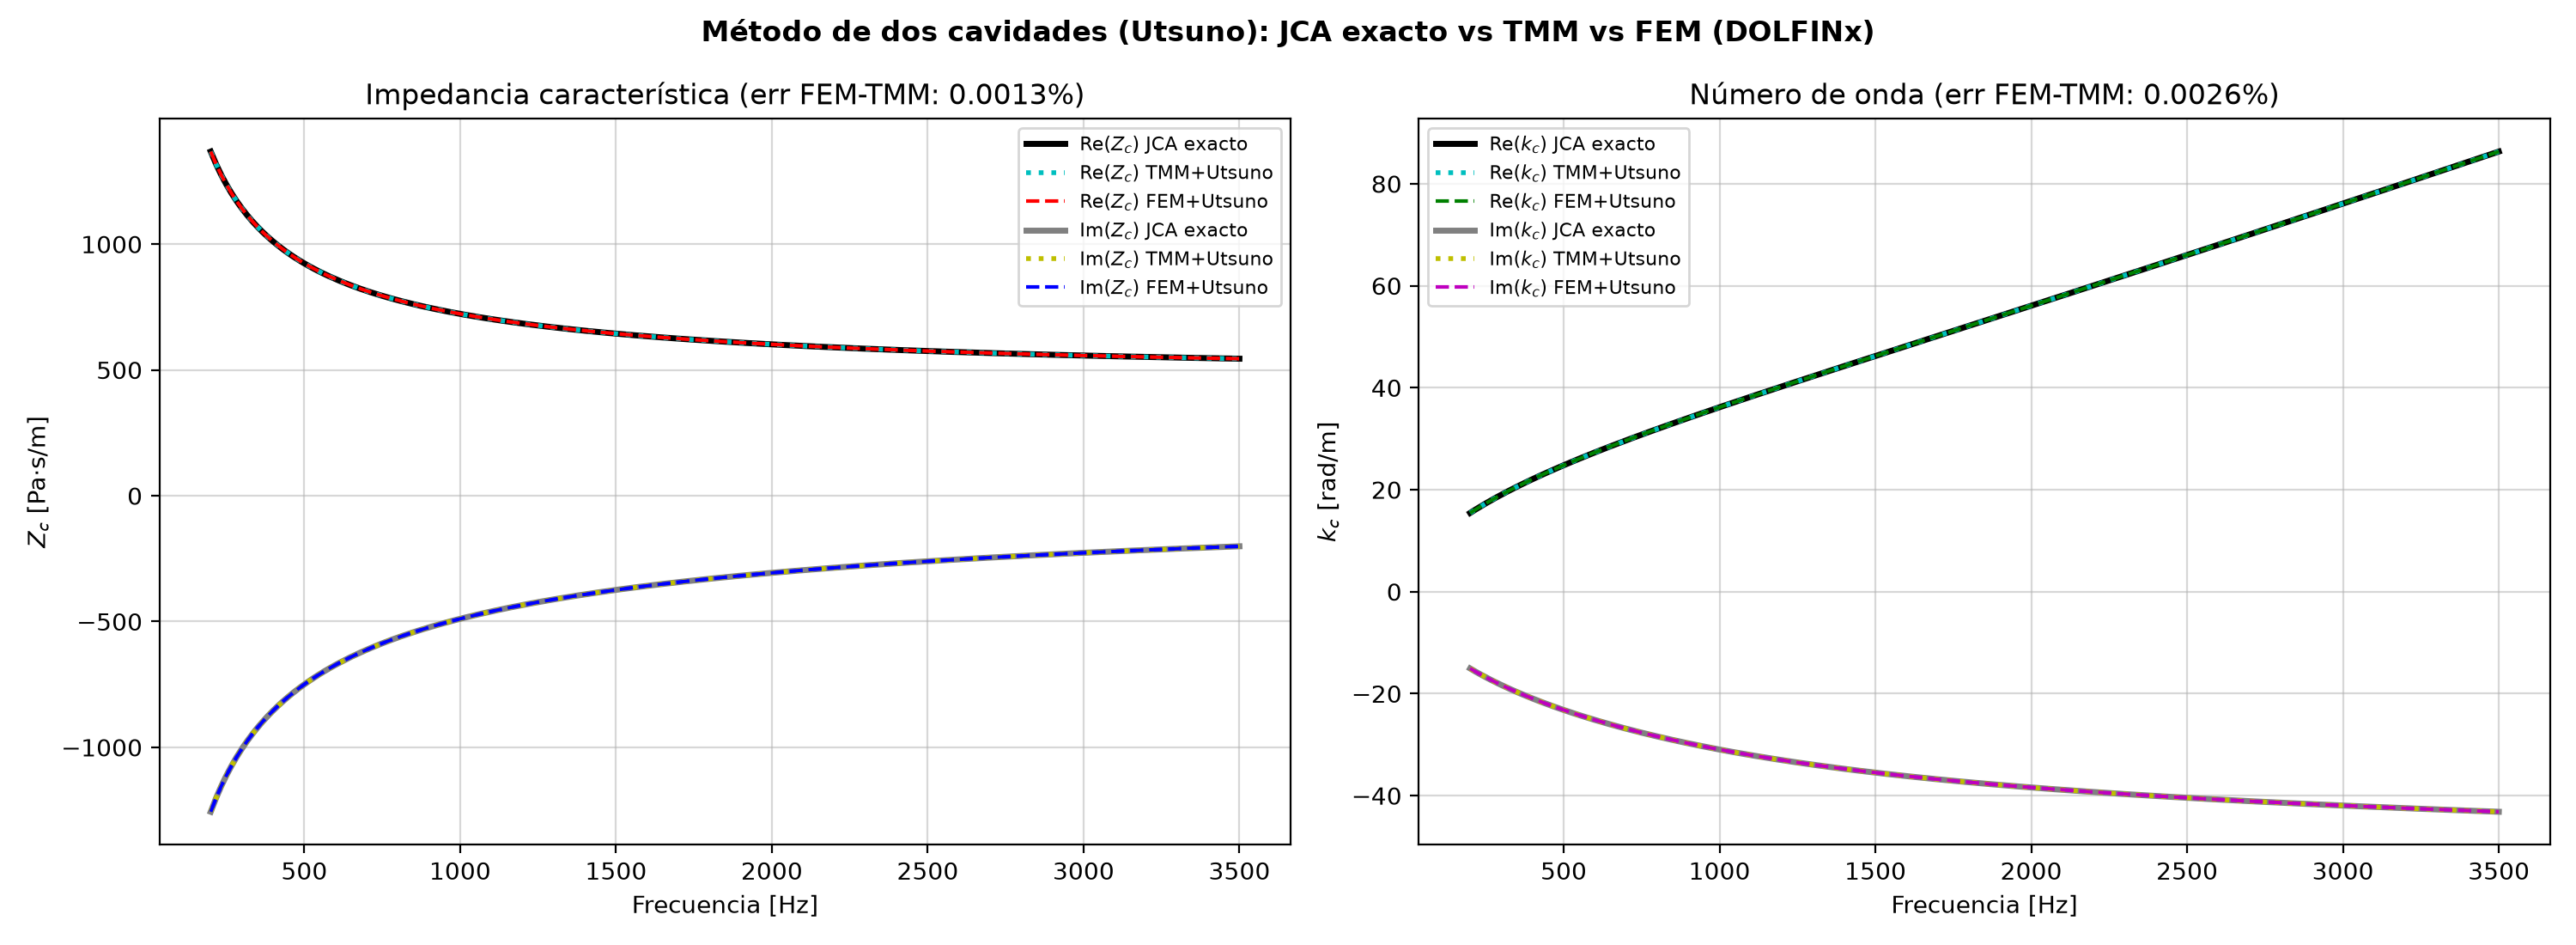
\includegraphics[width=\textwidth]{validacion_utsuno_tmm_fem_dolfinx.png}
\caption{Validación del método de dos cavidades: $Z_c$ (izquierda) y $k_c$ (derecha) del modelo JCA exacto, de TMM con Utsuno y de FEM (DOLFINx) con Utsuno. Parte real e imaginaria.}
\label{fig:validacion}
\end{figure}

\begin{table}[ht]
\centering
\caption{Error relativo global entre las reconstrucciones FEM y TMM.}
\label{tab:errores}
\begin{tabular}{@{}lc@{}}
\toprule
\textbf{Magnitud} & \textbf{Error relativo (FEM vs. TMM)} \\
\midrule
Impedancia característica $Z_c$ & $0{,}0013\ \%$ \\
Número de onda complejo $k_c$ & $0{,}0026\ \%$ \\
\bottomrule
\end{tabular}
\end{table}

El error entre ambas vías es del orden de $10^{-3}\,\%$ (Tabla~\ref{tab:errores}), lo que valida la formulación débil, las condiciones de contorno (radiación con fuente y cavidad rígida), el procesamiento de dos micrófonos y la implementación en DOLFINx. Este nivel de error es consistente con el de discretización de los elementos P1 en la malla utilizada. Por su parte, la reconstrucción TMM con Utsuno recupera el modelo JCA con un error inferior a $10^{-5}\,\%$, lo que confirma que el algoritmo inverso es correcto y que la diferencia observada proviene únicamente de la discretización numérica.

% =============================================================================
% SECCIÓN 6: IMPLEMENTACIÓN COMPUTACIONAL (SECCIÓN LIBRE PARA EL CÓDIGO)
% =============================================================================
\section{Implementación Computacional}
\label{sec:codigo}

A continuación se presenta el código completo en Python (FEniCSx/DOLFINx en modo complejo) que implementa el modelo JCA, el TMM, la solución por elementos finitos, el procesamiento de dos micrófonos y el algoritmo de Utsuno.

% --- Opción A: pegar el código directamente entre \begin{lstlisting} y \end{lstlisting}
% --- Opción B: descomentar la línea siguiente (el .py debe estar en la misma carpeta)
% \lstinputlisting[language=Python]{JCA_TMMUtsuno_FEMUtsuno_dolfinx.py}
\begin{lstlisting}[language=Python]
# >>> AQUÍ VA EL CÓDIGO SI FUESE NECESARIO <<<
\end{lstlisting}


% =============================================================================
% CONCLUSIONES
% =============================================================================
\section{Conclusiones}

La metodología integrada permite una caracterización completa y unívoca del material poroso. La validación numérica confirma la concordancia entre el modelo constitutivo JCA, la formulación discreta en FEniCSx bajo ISO 10534-2 y la reconstrucción analítica por el método de dos cavidades de Utsuno.

\end{document}